\section{Pointwise bounds without zeros}\label{sec:pointwise}

The sum rule bounds a mean. For zero-free systems with an affine phase on
the band there is a stronger statement: one explicit system has the least
attenuation at every frequency of the band at once. The proof writes every
admissible $h$ as the function $h_g$ of \cref{prop:profile} plus terms, one
for each unit of measure off the band, each of which raises the attenuation
at every point of the band.\footnote{The decomposition is the sum rule of
\cref{sec:sumrule} read pointwise: the weight $W$ of \cref{lem:kernel} is
replaced by the kernels $k_0$, $k_t$ of \cref{lem:atoms}, which are positive
at every point of the band.}

Throughout, $\Sigma=(0,a)\cup(b,\infty)$ is the part of the positive axis
off the band, and $\mu_0=\mu(\{0\})$. Put
\begin{gather*}
\tau_\circ=\frac{2K(k)}{\pi b}=\frac{\tau_\star}\theta,\qquad
h_\circ=\frac{h_\star}\theta,\qquad A=\frac{\alpha_\star}\theta,
\end{gather*}
so that $h_\circ$ is the extremal function of \cref{thm:extremal} for
$\theta=1$, with linear coefficient $\tau_\circ$ and attenuation
$A(x)=\tau_\circ\int_a^x(m^2-s^2)\dd s/r(s)$ on the band.

\subsection{One unit of measure off the band}

For $t\in\Sigma$ and $a<x<b$ put
\begin{gather*}
K_0(z)=\frac{R(z)}{abz},\qquad
K_t(z)=\frac{2zR(z)}{R(t)\,(t^2-z^2)},\\
k_0(x)=\frac{r(x)}{abx},\qquad
k_t(x)=\frac{2x\,r(x)}{R(t)\,(t^2-x^2)} .
\end{gather*}
By \cref{lem:R}, $R(t)$ and $t^2-x^2$ have the same sign for $t\in\Sigma$,
so $k_0>0$ and $k_t>0$ on $(a,b)$.

\begin{lemma}\label{lem:atoms}
$K_0$ and $K_t$, $t\in\Sigma$, are odd, analytic in $\C\setminus(S\cup\{0,\pm t\})$,
real on $\R\setminus S$ away from their poles, and
\begin{align*}
K_0(z)&=\frac z{ab}-\frac1z+\frac1\pi\int_a^b\frac{2z\,k_0(s)}{s^2-z^2}\dd s,\\
K_t(z)&=-\frac{2z}{R(t)}+\frac{2z}{t^2-z^2}
+\frac1\pi\int_a^b\frac{2z\,k_t(s)}{s^2-z^2}\dd s .
\end{align*}
On the band $\Re K_0(x+i0)=\Re K_t(x+i0)=0$, $\Im K_0(x+i0)=k_0(x)$ and
$\Im K_t(x+i0)=k_t(x)$.
\end{lemma}

\begin{proof}
The parity and reality follow from \cref{lem:R}, and the boundary values on
the band from $R(x+i0)=ir(x)$. Call $D$ the difference of the two sides of
either identity. At infinity $R(z)=z^2+O(1)$, so $K_0=z/(ab)+O(z^{-1})$ and
$K_t=-2z/R(t)+O(z^{-1})$, and the Cauchy integrals are $O(z^{-1})$; hence
$D=O(z^{-1})$. At $z=0$, $R(0)=-ab$, so $K_0=-1/z+O(z)$. At $z=\pm t$ the
residue of $K_t$ is $-1$, as is that of $2z/(t^2-z^2)$. So $D$ is analytic
off $S$. The Cauchy integral of the density $k/\pi$, $k=k_0$ or $k_t$,
which is H\"older continuous inside the band and of order $\abs{s-c}^{1/2}$
at its ends $c$, has the boundary imaginary part $k$ on $(a,b)$ by the
Plemelj formula, as in the proof of \cref{prop:profile}(ii), and is
continuous up to $S$ \cite[Ch.~4]{muskhelishvili}. Both sides of each
identity have imaginary part $k$ on the upper side of the band, so $D$ is
real there, and by the symmetry $D(\bar z)=\overline{D(z)}$ it takes the same
values from below. So $D$ has no jump across the open band, and by oddness none across $(-b,-a)$; it is bounded near
$\pm a,\pm b$, hence entire, and it tends to $0$. Thus $D=0$.
\end{proof}

\subsection{The reconstruction}

\begin{theorem}\label{thm:reconstruction}
Let $H=\sigma e^{ih}$ be a zero-free passive system, regular on the band,
whose phase $g=\varphi$ is continuously differentiable on $[a,b]$. Then
$\int_\Sigma\dd\mu(t)/\abs{R(t)}<\infty$ and
\begin{equation}\label{eq:reconstruction}
h=h_g+\mu_0K_0+\int_\Sigma K_t\dd\mu(t).
\end{equation}
Consequently, for $a<x<b$,
\begin{gather}
\alpha(x)=v_g(x)+\mu_0\,k_0(x)+\int_\Sigma k_t(x)\dd\mu(t),\label{eq:positive}\\
\beta=\beta_g+\frac{\mu_0}{ab}-\int_\Sigma\frac{2\dd\mu(t)}{R(t)} .\label{eq:betarec}
\end{gather}
\end{theorem}

The first identity says that the attenuation on the band is the
attenuation $v_g$ forced by the phase alone, plus a strictly positive
contribution of every unit of measure off the band. The second shows the
price of that measure in another currency: mass at frequencies below the
band, where $R<0$, raises the linear coefficient, and mass above the band
lowers it.

\begin{proof}
\emph{Finiteness.} For $t\to\infty$, $\abs{R(t)}\sim t^2$, and
$\int\dd\mu/(1+t^2)<\infty$. Near $a$ and $b$ the measure has a bounded
density by \cref{lem:regular}, and $\abs{R}^{-1}$ has singularities of
order $\abs{t-a}^{-1/2}$, $\abs{t-b}^{-1/2}$. Near $0$, $\abs R\ge ab/2$.

\emph{The right side.} Call it $\hat h$. Since $\abs{K_t(z)}$ is bounded by
a constant times $\abs{R(t)}^{-1}$ for $t\in\Sigma$ and $z$ in a compact set
at positive distance from $S\cup\{0\}\cup\operatorname{supp}\mu$, and for
$x$ in a compact subset of $(a,b)$ the same holds near $x+i0$, the integral
converges locally uniformly there; $\hat h$ is analytic off
$S\cup\{0\}\cup\operatorname{supp}\mu\cup-\operatorname{supp}\mu$ and
continuous up to the open band, where by \cref{prop:profile}(ii) and
\cref{lem:atoms} its real part is $g$. Integrating the identities of
\cref{lem:atoms} against $\mu$, by Fubini's theorem since every term is
absolutely integrable,
\[
\hat h(z)=\hat\beta z-\frac{\mu_0}z+\int_\Sigma\frac{2z}{t^2-z^2}\dd\mu(t)
+\frac1\pi\int_a^b\frac{2z\,\hat v(s)}{s^2-z^2}\dd s ,
\]
with $\hat\beta$ the right side of \eqref{eq:betarec} and $\hat v$ that of
\eqref{eq:positive}. Here we used that $h_g=\beta_gz+\frac1\pi\int_a^b
2zv_g(s)\dd s/(s^2-z^2)$: the difference of the two sides is odd, analytic
off $S$, $O(z^{-1})$ at infinity, continuous up to $S$, and has no jump
across the band, so it is entire and vanishes.

\emph{$\hat v$ is bounded.} $v_g$ is continuous on $[a,b]$ by
\cref{prop:profile}(i). In $\hat v(x)$ only the mass of $\mu$ near the band
edges can produce a singularity. For $x=a+\varepsilon$ and $t=a-u$ with
$0<u<\delta$, $k_t(x)$ is at most a constant times
$\sqrt\varepsilon/(\sqrt u\,(u+\varepsilon))$, and the density of $\mu$ is
bounded there, while
\[
\sqrt\varepsilon\int_0^\delta\frac{\dd u}{\sqrt u\,(u+\varepsilon)}\le\pi;
\]
the edge $b$ is the same. The rest of $\mu$ contributes a bounded amount by
the finiteness above.

\emph{Uniqueness.} By \eqref{eq:foster} and \cref{lem:regular},
$h=\beta z-\mu_0/z+\int_\Sigma2z\dd\mu/(t^2-z^2)+\frac1\pi\int_a^b2z\alpha(s)
\dd s/(s^2-z^2)$. So
\[
q=h-\hat h=(\beta-\hat\beta)z+\frac1\pi\int_a^b\frac{2z\,(\alpha-\hat v)(s)}{s^2-z^2}\dd s ,
\]
which is analytic off $S$, odd, $O(z)$ at infinity, and $O(\log\abs{z-c})$
near each end $c$ of $S$, because $\alpha-\hat v$ is bounded. Both $h$ and
$\hat h$ are continuous up to the open band with real part $g$, so, exactly
as in the proof of \cref{prop:profile}(iv), $q/R$ has the same boundary
values from both sides of $(a,b)$ and of $(-b,-a)$. It is therefore analytic
across the open cuts, its singularities at $\pm a,\pm b$ are
$o(\abs{z-c}^{-1})$ and hence removable, and $q/R$ is entire. At infinity
$q/R=O(z^{-1})$. Hence $q=0$, which is \eqref{eq:reconstruction}; comparing
linear coefficients and densities gives $\beta=\hat\beta$ and
$\alpha=\hat v$ almost everywhere, hence everywhere by continuity.
\end{proof}

\begin{corollary}\label{cor:compare}
Under the hypotheses of \cref{thm:reconstruction}, for $a<x<b$,
\[
\alpha(x)\ \ge\ v_g(x)+\frac{r(x)}x\,\max\{0,-\beta_g\}.
\]
\end{corollary}

\begin{proof}
For $0<t<a<x$, $x/(x^2-t^2)>1/x$, so $k_t(x)>2r(x)/(x\abs{R(t)})$. Put
\[
C_{\rm in}=\frac{\mu_0}{ab}+\int_{(0,a)}\frac{2\dd\mu(t)}{\abs{R(t)}},\qquad
C_{\rm out}=\int_{(b,\infty)}\frac{2\dd\mu(t)}{R(t)} ,
\]
both nonnegative. By \eqref{eq:positive},
$\alpha(x)\ge v_g(x)+\frac{r(x)}xC_{\rm in}+\int_{(b,\infty)}k_t(x)\dd\mu(t)$,
and by \eqref{eq:betarec} and $\beta\ge0$,
$C_{\rm in}\ge C_{\rm out}-\beta_g\ge-\beta_g$.
\end{proof}

\subsection{Affine phase}

For $g(t)=t$, \cref{prop:profile} gives $\beta_g=\frac2\pi\int_a^bt\dd t/r(t)=1$
and $v_g=0$, by the substitution $\sigma=t^2$ and Glauert's integral (proof
of \cref{lem:positivity}); hence $h_g=z$. By linearity and
\cref{prop:profile}(iv), the phase $\theta+\tau\omega$ has
\begin{equation}\label{eq:affinehg}
h_g=\theta h_\circ+\tau z,\qquad v_g=\theta A,\qquad \beta_g=\theta\tau_\circ+\tau .
\end{equation}
The function $R(z)/z=abK_0(z)$ has, by \cref{lem:atoms}, linear coefficient
$1$, an atom $ab$ at the origin and band attenuation $r(x)/x$.

\begin{theorem}\label{thm:affine}
Let $\theta\ge0$, $\tau\in\R$, and $C=\max\{0,-\theta\tau_\circ-\tau\}$. Every
zero-free passive system, regular on the band, with phase $\theta+\tau\omega$
on $(a,b)$ satisfies
\begin{equation}\label{eq:affinebound}
\alpha(x)\ \ge\ \theta A(x)+C\,\frac{r(x)}x\qquad(a\le x\le b).
\end{equation}
Equality holds throughout the band for
\[
h_{\rm opt}(z)=\theta h_\circ(z)+\tau z+C\,\frac{R(z)}z ,
\]
and equality at a single point of $(a,b)$ forces $h=h_{\rm opt}$.
\end{theorem}

\begin{proof}
The bound is \cref{cor:compare} with \eqref{eq:affinehg}, extended to the
ends by continuity. By \cref{lem:atoms} and \eqref{eq:affinehg},
$h_{\rm opt}$ has the form \eqref{eq:foster} with linear coefficient
$\theta\tau_\circ+\tau+C\ge0$, an atom $Cab\ge0$ at the origin, and the
measure $\pi^{-1}(\theta A+Cr/x)\dd x\ge0$ on the band and nothing else. So
it is a Herglotz function with the symmetry of \eqref{eq:Hh}, continuous up
to a neighbourhood of $[a,b]$, and $e^{ih_{\rm opt}}$ is admissible with
phase $\theta+\tau\omega$ and attenuation $\theta A+Cr/x$.

Suppose equality at $x_0\in(a,b)$. In the proof of \cref{cor:compare} each
inequality is then an equality at $x_0$. Since $k_t(x_0)>0$ for $t>b$, $\mu$
vanishes on $(b,\infty)$; since the comparison for $0<t<a$ is strict, $\mu$
vanishes on $(0,a)$; and $C_{\rm in}=\mu_0/(ab)$ equals $C$. By
\eqref{eq:reconstruction}, $h=\theta h_\circ+\tau z+CabK_0=h_{\rm opt}$.
\end{proof}

\begin{figure}[t]
\centering
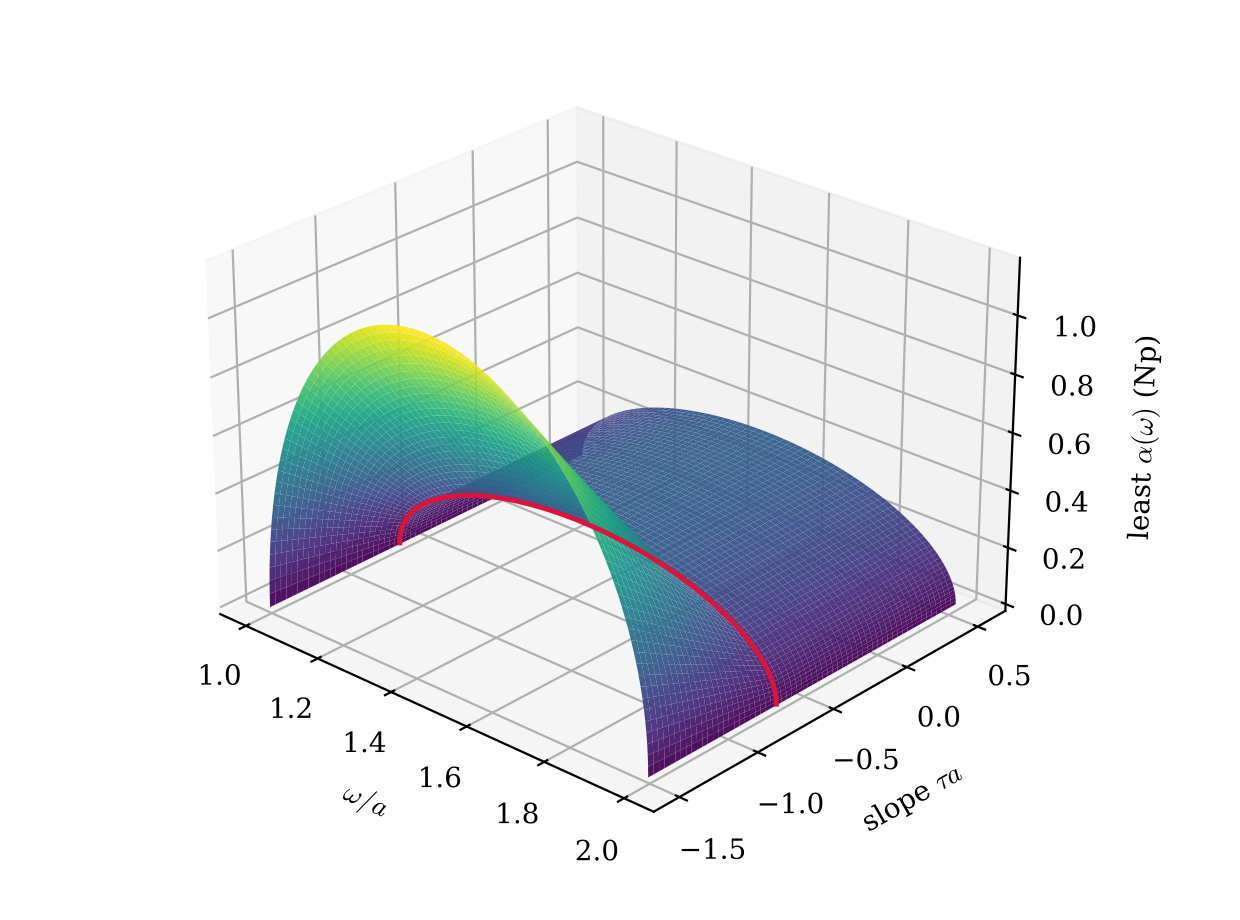
\includegraphics[width=\columnwidth]{figures/fig_pointwise.png}
\caption{The least attenuation $A(\omega)+\max\{0,-\tau_\circ-\tau\}\,r(\omega)/\omega$
of \cref{thm:affine} at each frequency of an octave, for the phase
$1+\tau\omega$, as a function of the slope $\tau$. For $\tau\ge-\tau_\circ$
(red curve at $\tau=-\tau_\circ=-0.6864/a$) it does not depend on $\tau$; below
it the pole at zero frequency adds $r(\omega)/\omega$ per unit of slope.}
\label{fig:pointwise}
\end{figure}

For $\tau\ge-\theta\tau_\circ$, in particular for a pure phase lag, the
optimum is $e^{i\tau z}H_\star$, and an additional delay costs nothing. A
negative slope beyond $-\theta\tau_\circ=-\tau_\star$ would make the linear
coefficient negative; the cheapest compensation, at every frequency of the
band at once, is then a pole of $h$ at zero frequency.

\subsection{Constant phase lead}

\begin{lemma}\label{lem:leadprofile}
$h_\circ(-ab/z)=-h_\circ(z)+\tau_\circ R(z)/z$. Consequently
\[
A(ab/x)=\tau_\circ\frac{r(x)}x-A(x)>0\qquad(a<x<b).
\]
\end{lemma}

\begin{proof}
The function $f(z)=h_\circ(-ab/z)$ is a Herglotz function with the symmetry
of \eqref{eq:Hh}, regular on the band, as in the proof of \cref{thm:lead};
its phase on the band is $-1$ and its attenuation is $A(ab/x)$. Since
$h_\circ$ is analytic at $0$ with $h_\circ(0)=0$, $f$ has linear coefficient
$0$; since $h_\circ(w)=\tau_\circ w+O(w^{-1})$, $f(z)=-\tau_\circ ab/z+O(z)$
near $0$, an atom $\tau_\circ ab$; and $f$ is real on $\Sigma$, so $\mu$ has
no other mass there. \Cref{thm:reconstruction} with $g=-1$, for which
$h_g=-h_\circ$, gives $f=-h_\circ+\tau_\circ abK_0$. Taking imaginary parts
on the band gives the second identity; $A(ab/x)>0$ by \cref{thm:extremal}(ii).
\end{proof}

\begin{theorem}\label{thm:leadpoint}
Let $s>0$ and $\tau\le0$. Every zero-free passive system, regular on the
band, with phase $-s+\tau\omega$ on $(a,b)$ satisfies
\[
\alpha(x)\ \ge\ s\,A(ab/x)-\tau\,\frac{r(x)}x\qquad(a\le x\le b),
\]
with equality throughout the band for
$h=-sh_\circ+\tau z+(s\tau_\circ-\tau)R/z$, and equality at one point of
$(a,b)$ forces this $h$. For $\tau=0$ the optimum is $H_\star(-ab/z)$ with
$H_\star$ the extremal system for $\theta=s$.
\end{theorem}

\begin{proof}
Here $v_g=-sA$ and $\beta_g=-s\tau_\circ+\tau<0$, so \cref{cor:compare} and
\cref{lem:leadprofile} give $\alpha\ge-sA+(s\tau_\circ-\tau)r/x
=sA(ab/x)-\tau r/x$. The stated $h$ has linear coefficient $0$, an atom
$(s\tau_\circ-\tau)ab>0$ at the origin and band density
$\pi^{-1}(sA(ab/x)-\tau r/x)>0$, so it is admissible. Equality at one point
forces $h$ as in the proof of \cref{thm:affine}. For $\tau=0$,
\cref{lem:leadprofile} identifies $h$ with $sh_\circ(-ab/z)$.
\end{proof}

\subsection{Consequences}

\begin{corollary}\label{cor:pointwisecons}
\begin{enumerate}
\item[(i)] For phase $\theta+\tau\omega$ with $\theta\ge0$, $\tau\in\R$, or
with $\theta<0$, $\tau\le0$, the optimal system of
\cref{thm:affine,thm:leadpoint} minimises $\int_a^bw\,\alpha$ for every
weight $w\ge0$, every $L^p$ norm of $\alpha$ on the band, $1\le p\le\infty$,
and every functional of $\alpha$ that increases with $\alpha$; for
$\int w\alpha$ with $w\ne0$ it is the only minimiser.
\item[(ii)] For phase $\theta\ge0$, the least value of $\max_{[a,b]}\alpha$ is
$\theta A(m)=\alpha_\star(m)$; for phase $-s<0$ it is $sA(m)$, attained at
$x=ab/m$.
\item[(iii)] For phase $-s<0$ the least mean attenuation over the band is
$s\Lambda_-$, with
\[
\Lambda_-=\frac{E(\kappa)-\kappa'^2K(\kappa)}{\kappa},\qquad\kappa'^2=1-\kappa^2 .
\]
\item[(iv)] For phase $\theta+\tau\omega$ with $\theta\ge0$ and
$\tau<-\tau_\star$, the least mean attenuation is
\[
\theta\Lambda+\frac\pi4\,(b-a)\,(-\tau-\tau_\star).
\]
\end{enumerate}
\end{corollary}

\begin{proof}
(i) follows from the pointwise bounds and their equality cases; a weight
$w\ge0$ that is not almost everywhere zero is positive on a set of positive
measure, where any other admissible system has strictly larger
attenuation, by the equality cases and continuity. (ii) $A$ is largest at
$m$ (\cref{thm:extremal}(ii)). (iii) is the value computed in
\cref{rem:leadmean} for $H_\star(-ab/z)$. (iv) Integrate
\eqref{eq:affinebound} with $C=-\tau-\tau_\star$, using
\[
\int_a^b\frac{r(x)}x\dd x=\frac\pi4(b-a)^2 ,
\]
which follows from $\sigma=x^2$, $A=a^2$, $B=b^2$ and the substitution
$\sigma=c-d\cos\phi$, $c=\frac{A+B}2$, $d=\frac{B-A}2$:
\begin{align*}
\int_A^B\frac{\sqrt{(\sigma-A)(B-\sigma)}}\sigma\dd\sigma
&=d^2\int_0^\pi\frac{\sin^2\phi\,\dd\phi}{c-d\cos\phi}\\
&=\pi\big(c-\sqrt{c^2-d^2}\big)\\
&=\frac\pi2\big(\sqrt B-\sqrt A\big)^2 ,
\end{align*}
since $c^2-d^2=AB$.
\end{proof}

For an octave $A(m)=0.34824$, so the least worst-frequency attenuation for a
lag $\theta$ is $1.2731\,\theta\Lambda$, against the mean $\theta\Lambda=0.27353\,\theta$;
and $\Lambda_-=0.26560$. So the sharp worst-frequency bound for a lag and the sharp plain mean for
a lead are both attained by the extremal system or by its inversion.

\begin{figure}[t]
\centering
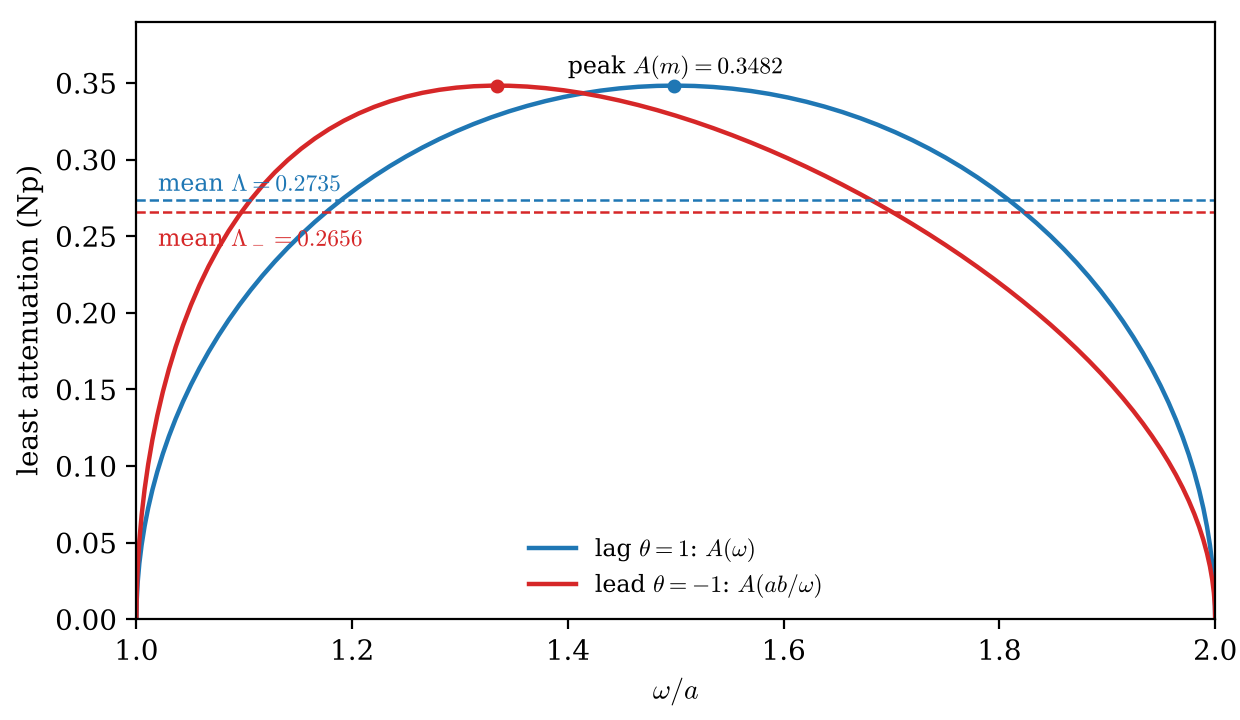
\includegraphics[width=\columnwidth]{figures/fig_leadlag.png}
\caption{The least attenuation at each frequency of an octave for a unit
lag (\cref{thm:affine}) and a unit lead (\cref{thm:leadpoint}). The lead
profile is the lag profile reflected by $\omega\mapsto ab/\omega$; the two
have the same peak $A(m)$, at $m$ and at $ab/m$, and different means.}
\label{fig:leadlag}
\end{figure}

\subsection{A prescribed argument}

\begin{theorem}\label{thm:branches}
Let $0<\vartheta<\pi$. Among zero-free passive systems regular on the band
with $\arg H\equiv\vartheta$ modulo $2\pi$ on $[a,b]$, the least mean
attenuation is $\min\{\vartheta\Lambda,(\pi-\vartheta)\Lambda_-\}$ and the
least value of $\max_{[a,b]}\alpha$ is $\min\{\vartheta,\pi-\vartheta\}A(m)$.
\end{theorem}

\begin{proof}
By \cref{rem:arg} the phase is a constant $\theta'\equiv\vartheta\pmod\pi$.
If $\theta'>0$ then $\theta'\ge\vartheta$, and by \cref{thm:main} and
\cref{cor:pointwisecons}(ii) both costs are at least $\vartheta\Lambda$ and
$\vartheta A(m)$, with equality for $H_\star$ with $\theta=\vartheta$. If
$\theta'<0$ then $\abs{\theta'}\ge\pi-\vartheta$, and
\cref{cor:pointwisecons}(ii), (iii) give $(\pi-\vartheta)\Lambda_-$ and
$(\pi-\vartheta)A(m)$, attained by $-H_\star(-ab/z)$ with $\theta=\pi-\vartheta$.
\end{proof}

So the mean is least on the lagging branch for
$\vartheta<\vartheta_c=\pi\Lambda_-/(\Lambda+\Lambda_-)$ and on the leading
branch beyond it, while the worst frequency changes branch at $\pi/2$. For an
octave $\vartheta_c=1.5477$, just below $\pi/2$: the two costs prefer
different systems for $\vartheta_c<\vartheta<\pi/2$. \Cref{thm:branches}
sharpens \cref{cor:worst}, whose constant $\Lambda$ becomes $A(m)$.
